% =============================================================================
% Chapter 4: System Design and Architecture
% NexaLearn Graduation Project — Cairo University, Faculty of Engineering
% =============================================================================

\chapter{System Design and Architecture}
\label{ch:system-design}

This chapter presents the complete system design and architectural blueprint of the NexaLearn platform. The design is grounded in the Domain-Driven Design and Clean Architecture principles surveyed in Chapter~3, and directly addresses the problem sub-problems identified in Chapter~1: lack of vertical coverage in open backends, unreliable asynchronous event processing, architectural erosion across many bounded contexts, and exactly-once semantics for financial and AI integrations.

The chapter begins with a high-level overview and the assumptions that constrain the design space (Section~\ref{sec:overview-assumptions}). Section~\ref{sec:sys-arch} presents the layered architecture block diagram and the module dependency graph, including a comprehensive summary table of all fifteen bounded contexts. The subsequent sections examine each module in depth: authentication (Section~\ref{sec:auth-module}), course management (Section~\ref{sec:course-module}), media and video processing (Section~\ref{sec:media-module}), AI pipeline integration (Section~\ref{sec:ai-pipeline-module}), assessment and quizzes (Section~\ref{sec:assessment-module}), payments (Section~\ref{sec:payment-module}), enrollment (Section~\ref{sec:enrollment-module}), and discussion (Section~\ref{sec:discussion-module}). Each module section follows a consistent structure: functional description, state machine, data flow, key entities, and design decisions. Section~\ref{sec:security-design} concludes the chapter with cross-cutting security mechanisms including HMAC service-to-service authentication, rate limiting, and audit logging.

Every module description includes a state machine diagram and references to the corresponding implementation artefacts in the NestJS codebase. Code listings highlight the domain entity behaviours that enforce business invariants at the aggregate root level.

% =============================================================================
% Section 4.1: Overview and Assumptions
% =============================================================================

\section{Overview and Assumptions}
\label{sec:overview-assumptions}

NexaLearn is designed as a \textbf{modular monolith}: a single NestJS application process that hosts fifteen bounded contexts, each mapped to a NestJS module (or a coherent group of modules) following the DDD tactical patterns and Clean Architecture layering described in Section~\ref{sec:ddd-clean-arch}. The system is deployed via Docker Compose with PostgreSQL as the primary data store and Redis as the session cache, rate-limiter backing store, and real-time pub/sub channel for progress events.

The following assumptions constrain the design and are validated by the target customer segments identified in Section~\ref{sec:targeted-customers}:

\begin{enumerate}
  \item \textbf{Concurrent learner count.} The platform is designed for 500--5,000 concurrently active learners per deployment instance, corresponding to a mid-size university department or a growth-stage edtech startup. Peak read load is estimated at 1,000 requests per second; peak write load at 200 events per second. This profile justifies the modular monolith deployment model over a microservices architecture, as the expected throughput does not require independent horizontal scaling per service.
  \item \textbf{Course catalogue size.} The system supports up to 500 active courses, each containing up to 50 lessons. Total video asset storage is assumed to be under 5 TB, managed by Mux's cloud transcoding and CDN delivery rather than self-hosted storage.
  \item \textbf{Network reliability.} External provider webhooks (Stripe, Mux, AI pipeline callbacks) may be delivered at-least-once, potentially with duplicates or out-of-order delivery. The system must tolerate these without producing incorrect state.
  \item \textbf{Instructor technical literacy.} Instructors are assumed to be domain experts (professors, corporate trainers) who can upload video files and review AI-generated quizzes via a web dashboard, but are not expected to write code, manage servers, or configure infrastructure.
  \item \textbf{Idempotency requirement.} All external-facing write endpoints and event handlers must be idempotent, allowing safe retry by clients or webhook senders.
\end{enumerate}

These assumptions shape the architectural decisions presented throughout this chapter. Where an assumption is violated by a specific deployment scenario (e.g., a large university with 50,000 students), the architecture provides documented migration paths: extracting the modular monolith into microservices (Section~\ref{sec:implemented-approach}), adding a message broker for higher event throughput, and deploying read replicas for analytics queries.

% =============================================================================
% Section 4.2: System Architecture
% =============================================================================

\section{System Architecture}
\label{sec:sys-arch}

\subsection{High-Level Architecture Block Diagram}
\label{subsec:arch-block-diagram}

Figure~\ref{fig:system-arch} presents the layered architecture of NexaLearn following the Dependency Rule of Clean Architecture. The outermost layer (Presentation) handles HTTP concerns through NestJS controllers, guards, pipes, and interceptors. The Application layer contains use-case interactors that orchestrate domain objects without depending on infrastructure. The Domain layer holds entities, aggregates, value objects, domain events, and repository port interfaces in pure TypeScript with zero framework dependencies. The Infrastructure layer implements the repository ports using Prisma, Stripe SDK, Mux SDK, Redis client, and AWS S3 SDK. A shared Events module provides the transactional outbox publisher and the in-process event bus.

\begin{figure}[H]
  \centering
  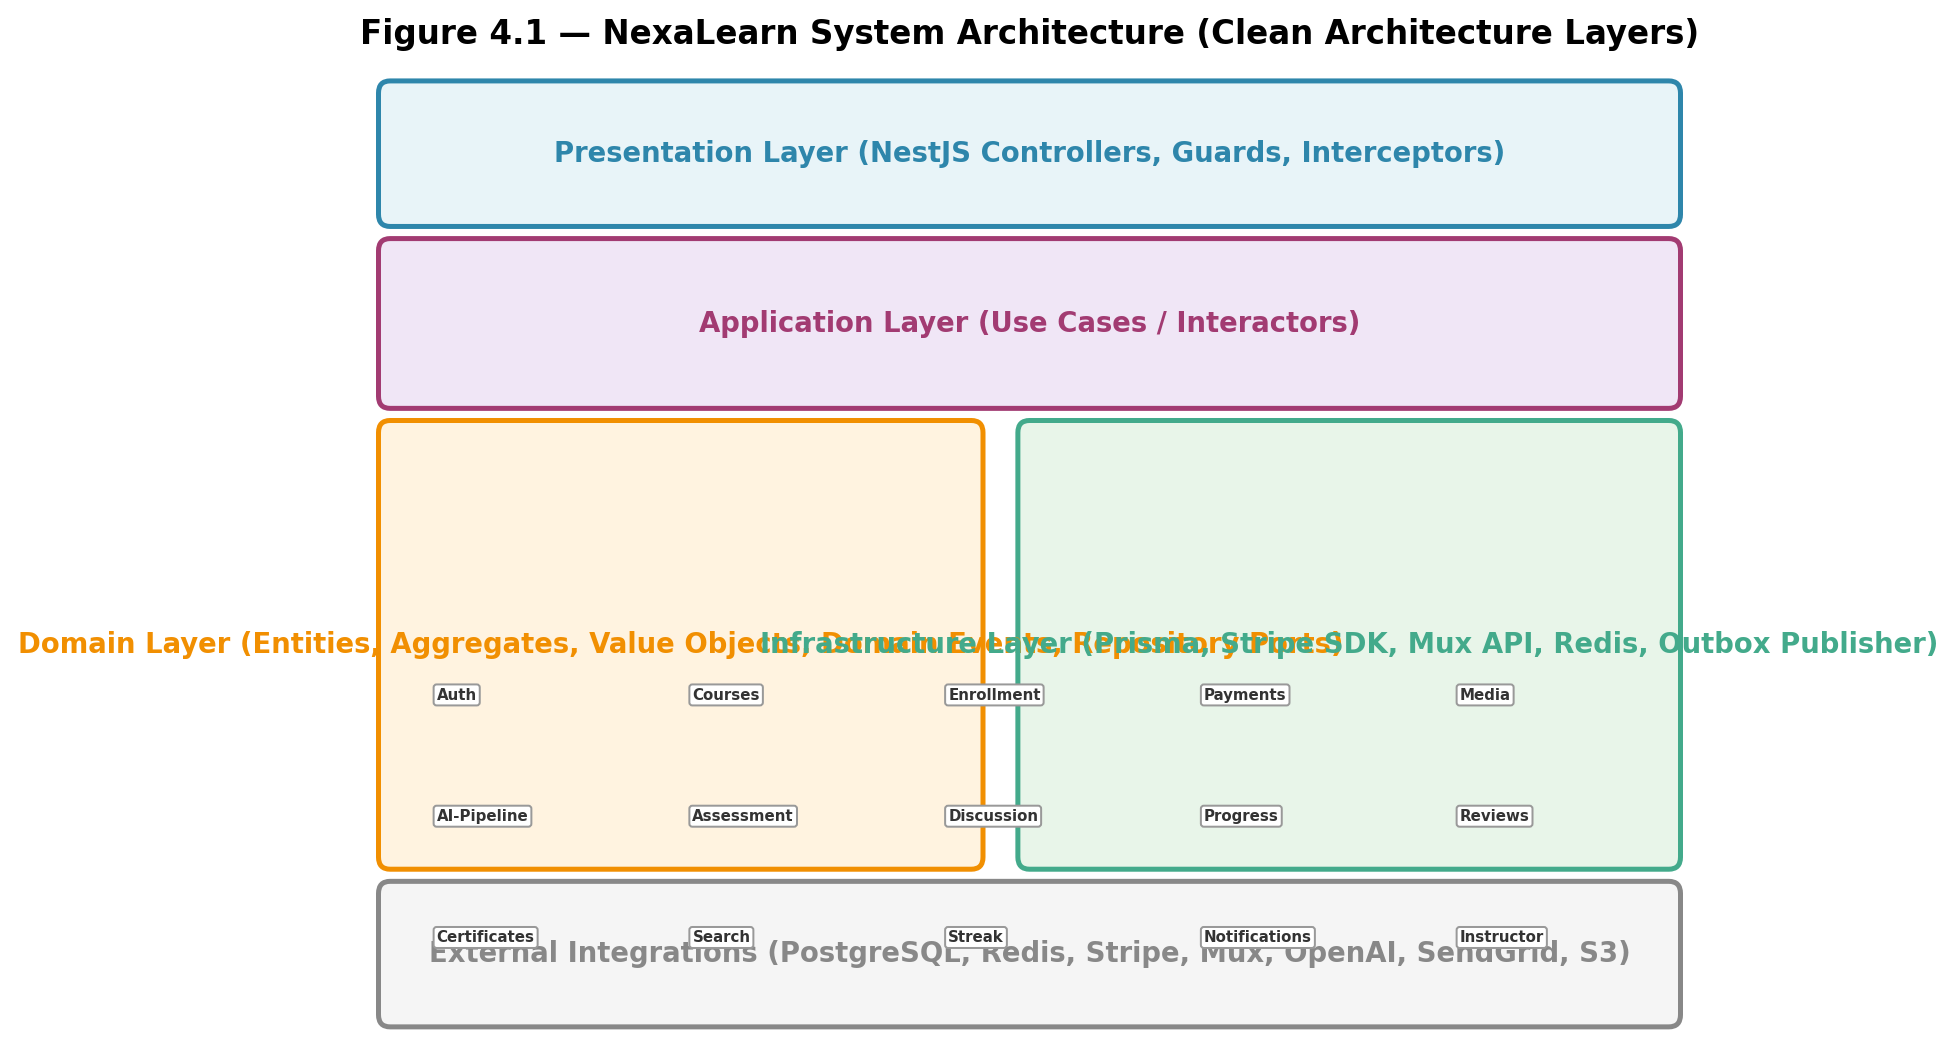
\includegraphics[width=\textwidth]{images/system_arch.png}
  \caption{NexaLearn System Architecture --- Clean Architecture Layers}
  \label{fig:system-arch}
\end{figure}

The Presentation layer routes HTTP requests to the appropriate Application use case. For example, a POST request to \texttt{/api/enrollments} is received by \texttt{EnrollmentController}, validated by a NestJS \texttt{ValidationPipe} using class-validator DTOs, and delegated to \texttt{CreateEnrollmentUseCase}. The use case loads the relevant domain aggregates (Course, User), enforces business rules (course is published, user is not already enrolled), creates a new \texttt{Enrollment} aggregate, and persists it through an \texttt{EnrollmentRepository} port. The repository implementation in Infrastructure writes to PostgreSQL via Prisma and---within the same transaction---inserts an outbox event for \texttt{EnrollmentCreated}. The outbox processor subsequently publishes this event to downstream consumers (Progress, Notifications, Search).

\subsection{Module Dependency Graph}
\label{subsec:module-dependency}

Figure~\ref{fig:module-interaction} shows the dependency and event-flow relationships among the fifteen bounded contexts. Solid arrows represent direct method-call dependencies (use cases in one context invoking repository or query service interfaces exported by another). Dashed arrows represent event-driven communication through the outbox: the source context publishes an event that is consumed by the target context's event handler.

\begin{figure}[H]
  \centering
  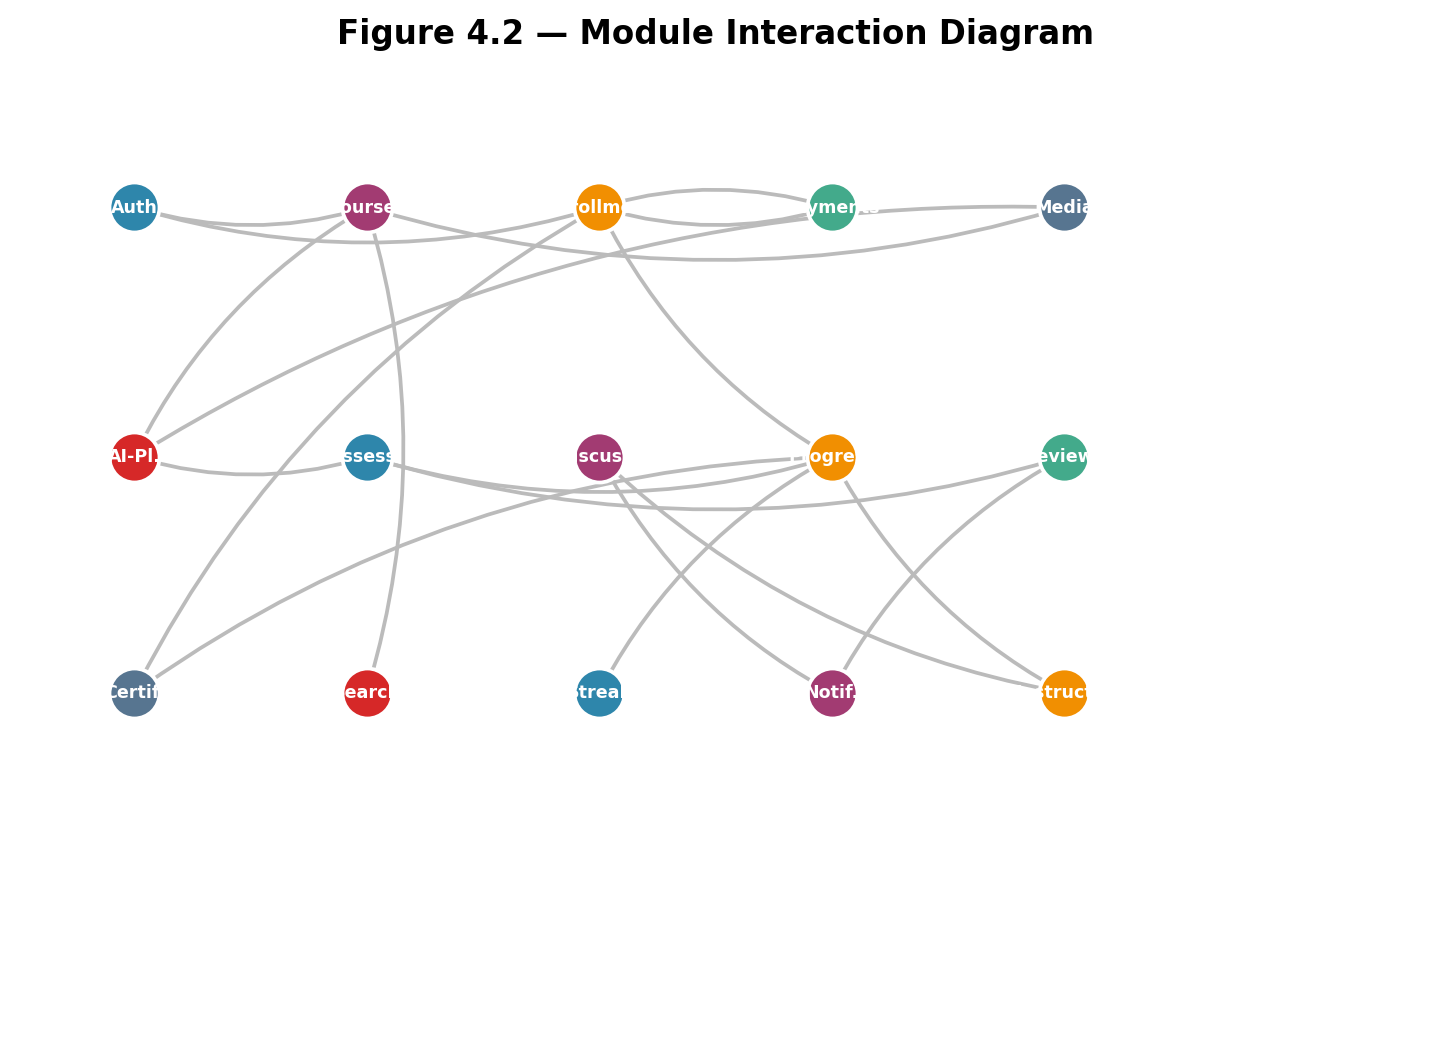
\includegraphics[width=0.8\textwidth]{images/module_interaction.png}
  \caption{NexaLearn Module Interaction Diagram}
  \label{fig:module-interaction}
\end{figure}

The diagram reveals several structural patterns. \textbf{Enrollment} acts as a hub, depending on Payments for payment verification and on Progress for projection initialisation. \textbf{Courses} depends on Media for video asset management and on AI-Pipeline for transcript and quiz generation. \textbf{Assessment} publishes graded-quiz events consumed by Progress and Reviews. \textbf{Notifications} is a pure consumer: it subscribes to events from Discussion, Reviews, and AI-Pipeline without exposing any outward-facing dependencies. \textbf{Instructor/Analytics} is a read-heavy context that queries read models built by Progress, Assessment, and Streak, and has no write-side dependencies.

\subsection{Module Summary}
\label{subsec:module-summary}

Table~\ref{tab:module-summary} enumerates all fifteen bounded contexts with their primary entities, published events, and module dependencies. This table serves as a quick reference for the detailed module descriptions that follow in Sections~\ref{sec:auth-module} through~\ref{sec:discussion-module}.

\begin{longtable}{@{}p{2.0cm} p{1.8cm} p{3.2cm} p{3.2cm} p{2.8cm}@{}}
  \caption{Module Summary --- Bounded Contexts, Entities, Events, and Dependencies}
  \label{tab:module-summary} \\
  \toprule
  \textbf{Module} & \textbf{Context} & \textbf{Key Entities} & \textbf{Key Events} & \textbf{Depends On} \\
  \midrule
  \endhead
  \midrule
  \endfoot
  Auth & Auth & User, RefreshTokenSession & UserLoggedIn, UserLoggedOut, SessionRevoked & --- \\
  \addlinespace
  Courses & Courses & Course, CourseModule, Lesson, Category & CoursePublished, LessonUpdated, CourseArchived & Media, AI-Pl. \\
  \addlinespace
  Enrollment & Enrollment & Enrollment, EnrollmentEvent & EnrollmentActivated, EnrollmentCancelled, EnrollmentCompleted & Payments, Courses \\
  \addlinespace
  Payments & Payments & PaymentIntent, PaymentTransaction, Refund & PaymentSucceeded, PaymentFailed, PaymentRefunded & Stripe (ext.) \\
  \addlinespace
  Media & Media & VideoAsset, UploadUrl, PlaybackToken & VideoUploaded, VideoReady, VideoErrored & Mux (ext.) \\
  \addlinespace
  AI-Pipeline & AI-Pipeline & GenerationJob, Transcript, GeneratedQuiz & JobCompleted, CallbackReceived, QuizReadyForReview & Media, OpenAI (ext.) \\
  \addlinespace
  Assessment & Assessment & Quiz, Question, QuestionOption, QuizAttempt, ShortAnswerGrade & QuizAttemptSubmitted, AttemptGraded, QuizPublished & Courses, AI-Pl. \\
  \addlinespace
  Discussion & Discussion & Thread, Post, ThreadInstructorReply & ThreadCreated, PostAdded, InstructorReplied & --- \\
  \addlinespace
  Progress & Progress & CourseProgressView, LessonProgress, ResumeView, LessonAnalytics & ProgressUpdated, LessonCompleted, StreakUpdated & Enrollment, Assessment \\
  \addlinespace
  Reviews & Reviews & Review, ReviewVote & ReviewSubmitted, ReviewFlagged & Assessment \\
  \addlinespace
  Certificates & Certificates & Certificate, CertificateTemplate & CertificateIssued, CertificateRevoked & Enrollment, Progress \\
  \addlinespace
  Search & Search & CourseSearchIndex, LessonSearchIndex & SearchIndexUpdated & Courses \\
  \addlinespace
  Streak & Streak & StreakRecord, StreakMilestone & StreakIncremented, StreakMilestoneReached & Progress \\
  \addlinespace
  Notifications & Notifications & Notification, EmailTemplate, NotificationPreference & NotificationSent, EmailDelivered, EmailBounced & Auth, Discussion, Assessment, Payments \\
  \addlinespace
  Instructor & Instructor & InstructorAnalyticsView, InstructorDashboard & --- (read-only) & Progress, Assessment, Streak \\
  \bottomrule
\end{longtable}

The next eight sections examine the core modules---Auth, Courses, Media, AI-Pipeline, Assessment, Payments, Enrollment, and Discussion---in architectural depth. Each section includes the domain aggregate design, state machine diagram, key code listings, and the design trade-offs that shaped the implementation.

% =============================================================================
% Section 4.3: Authentication and Session Management Module
% =============================================================================

\section{Authentication and Session Management Module}
\label{sec:auth-module}

\subsection{Functional Description}

The Auth module handles user registration, credential-based login, token issuance, session management, and logout. It implements a dual-token JWT architecture with server-side refresh token rotation and reuse detection, following best practices for mitigating token theft described by the IETF OAuth 2.0 Security BCP. The module depends on Redis for storing refresh token sessions and on PostgreSQL for persistent user records.

All authentication flows assume HTTPS transport. Tokens are opaque to clients in the sense that the access token contains only claims necessary for authorisation (user ID, role, expiration); no sensitive data is embedded. The refresh token is an opaque UUID that serves as a key into the Redis session store.

\subsection{JWT Token Architecture}

The system issues two token types:

\begin{description}
  \item[\textbf{Access Token.}] A short-lived (15-minute) JWT signed with an RS256 private key. The token encodes: \texttt{sub} (user ID), \texttt{role} (student, instructor, admin), \texttt{iat} (issued at), and \texttt{exp} (expiration). The access token is transmitted as \texttt{Authorization: Bearer <token>}. It is validated by a NestJS \texttt{AuthGuard} that verifies the RS256 signature using the corresponding public key, checks expiration, and attaches the decoded payload to the request context. No database lookup is performed on access token validation, enabling O(1) verification.
  \item[\textbf{Refresh Token.}] A 64-character cryptographically random string generated via \texttt{crypto.randomBytes(48)}. The refresh token is hashed using SHA-256 before storage; the raw token is returned to the client exactly once. The hashed token, along with the user ID, device metadata, and expiration timestamp (7 days), is stored in Redis under key \texttt{session:<hashed\_token>} with an appropriate TTL.
\end{description}

The separation of concerns mirrors the pattern used by Auth0 and Firebase Authentication: the access token is a stateless assertion verified by any service without a central session store, while the refresh token enables long-lived sessions without storing secrets on the client beyond the browser's secure, HTTPOnly cookie storage.

\subsection{Redis Session Store Design}

The Redis session store provides three operations:

\begin{enumerate}
  \item \textbf{Session creation.} On login, the system generates a refresh token, hashes it, and stores the session record: \texttt{SET session:<hash> user\_id=<uid> role=<role> device=<ua> created\_at=<ts> EX 604800}. The raw token is returned to the client.
  \item \textbf{Session validation.} On token refresh, the system hashes the provided refresh token, retrieves the session from Redis, and checks that the user ID matches and the session is not revoked. If valid, a new access--refresh token pair is issued and the old session is deleted.
  \item \textbf{Session revocation.} On logout or administrative revocation, the session key is deleted from Redis. Any subsequent attempt to use the associated refresh token fails validation.
\end{enumerate}

Redis is chosen over PostgreSQL for session storage because: (1) TTL-based expiration is native to Redis and eliminates the need for a session-cleanup cron job, (2) read latency is sub-millisecond compared to 1--5 ms for PostgreSQL, and (3) the session data is ephemeral---losing all sessions on a Redis restart is acceptable as users can re-authenticate.

\subsection{Refresh Token Rotation and Reuse Detection}

The Auth module implements refresh token rotation: each time a refresh token is used to obtain a new access token, the old refresh token is invalidated and a new one is issued. This limits the window of vulnerability if a refresh token is stolen---the attacker can use it only once before rotation invalidates it.

Reuse detection handles the edge case where both the legitimate client and an attacker attempt to use the same refresh token concurrently. The detection algorithm is:

\begin{lstlisting}[caption=Refresh Token Reuse Detection,label=lst:refresh-reuse]
async function refreshTokens(rawToken: string): Promise<TokenPair> {
  const hash = sha256(rawToken);
  const session = await redis.get(`session:${hash}`);
  if (!session) throw new UnauthorizedException('Session not found');

  await redis.del(`session:${hash}`);

  // Issue new tokens
  const newRawToken = crypto.randomBytes(48).toString('hex');
  const newHash = sha256(newRawToken);
  await redis.set(`session:${newHash}`, session, 'EX', 604800);

  const accessToken = await this.jwtService.signAsync({
    sub: session.userId,
    role: session.role,
  });

  return { accessToken, refreshToken: newRawToken };
}
\end{lstlisting}

If two requests arrive with the same refresh token, the first deletes the session and creates a new one; the second finds the session missing and returns an error. This forces the legitimate client to re-authenticate, which is a minor inconvenience compared to the alternative of an attacker maintaining persistent access.

The state machine diagram (Figure~\ref{fig:auth-statemachine}) illustrates the session lifecycle.

\begin{figure}[H]
  \centering
  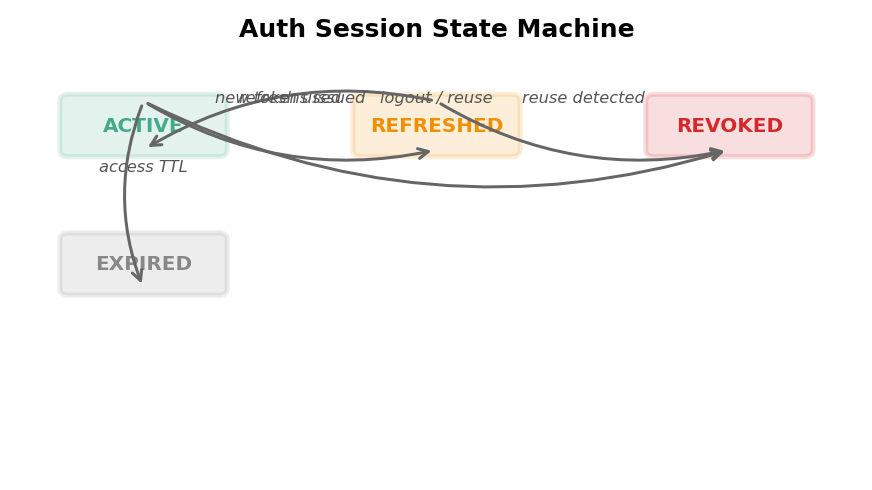
\includegraphics[width=0.65\textwidth]{images/statemachines/auth_session_statemachine.png}
  \caption{Auth Session State Machine}
  \label{fig:auth-statemachine}
\end{figure}

% =============================================================================
% Section 4.4: Course Management Module
% =============================================================================

\section{Course Management Module}
\label{sec:course-module}

\subsection{Functional Description}

The Courses module manages the curriculum lifecycle: instructors create courses, organise them into modules and lessons, attach video assets and quizzes to lessons, and publish the result for learner enrollment. The module is the content backbone of the platform, and its aggregate design must support deep nesting (course $\rightarrow$ module $\rightarrow$ lesson), reordering, versioning, and concurrent editing.

The module exposes REST endpoints for CRUD operations on courses, modules, and lessons, with dedicated endpoints for publishing/unpublishing, reordering, and category assignment.

\subsection{DDD Aggregate Design: Course--Module--Lesson Hierarchy}

The aggregate root is \texttt{CourseEntity}, which owns a collection of \texttt{CourseModuleEntity} value objects, each of which owns a collection of \texttt{LessonEntity} entities. The hierarchy is enforced by the aggregate root: all operations that modify modules or lessons must go through \texttt{CourseEntity} methods.

\begin{lstlisting}[caption=Course Aggregate Root,label=lst:course-aggregate]
export class CourseEntity {
  private constructor(
    public readonly id: string,
    public title: string,
    public description: string,
    public instructorId: string,
    public price: Money,
    public status: CourseStatus,
    public modules: CourseModuleEntity[],
    public version: number,
    public categoryId: string,
    public thumbnailUrl?: string,
  ) {}

  static create(props: CreateCourseProps): CourseEntity {
    return new CourseEntity(
      props.id, props.title, props.description,
      props.instructorId, props.price, CourseStatus.DRAFT,
      [], 1, props.categoryId,
    );
  }

  publish(): void {
    if (this.modules.length === 0)
      throw new BusinessRuleViolation('Course must have at least one module');
    if (this.modules.some(m => m.lessons.length === 0))
      throw new BusinessRuleViolation('Each module must have at least one lesson');
    if (!this.thumbnailUrl)
      throw new BusinessRuleViolation('Course must have a thumbnail');
    this.status = CourseStatus.PUBLISHED;
    this.version++;
  }

  reorderModules(moduleIds: string[]): void {
    const ordered = moduleIds.map(id => {
      const mod = this.modules.find(m => m.id === id);
      if (!mod) throw new BusinessRuleViolation(`Module ${id} not found`);
      return mod;
    });
    this.modules = ordered.map((m, i) => m.withPosition(i + 1));
    this.version++;
  }
}
\end{lstlisting}

The aggregate enforces three invariants at publication time: a course must have at least one module, every module must have at least one lesson, and a thumbnail must be set. These rules are checked in the \texttt{publish()} method and cannot be bypassed by external code.

\subsection{Optimistic Concurrency Control}

Each \texttt{CourseEntity} carries a \texttt{version} field that is incremented on every mutating operation. The Prisma repository implementation includes the version in the WHERE clause of the write query:

\begin{lstlisting}[caption=Optimistic Concurrency Update,label=lst:optimistic-lock]
async update(course: CourseEntity): Promise<void> {
  const result = await this.prisma.course.updateMany({
    where: { id: course.id, version: course.version - 1 },
    data: {
      title: course.title,
      status: course.status,
      modules: { deleteMany: {}, create: this.serializeModules(course) },
      version: course.version,
    },
  });

  if (result.count === 0)
    throw new ConcurrentModificationError(
      `Course ${course.id} was modified by another transaction`
    );
}
\end{lstlisting}

If two instructors open the same course, both modify it, and both submit their changes, the second write will match zero rows (because the version has been incremented by the first write) and the repository throws \texttt{ConcurrentModificationError}. The use case can catch this error and present the instructor with a conflict-resolution dialogue. This pattern avoids pessimistic locking (SELECT FOR UPDATE) which would block read access to course content during editing --- an unacceptable trade-off given that concurrent read access by enrolled learners is the common case.

\subsection{Idempotency for Lesson and Module Operations}

All mutating endpoints in the Courses module accept an optional \texttt{Idempotency-Key} header. The system maintains an idempotency ledger table (\texttt{course\_idempotency\_keys}) keyed by the SHA-256 hash of the key. If the same key is received within a configurable time window (default 24 hours), the response from the first request is returned without re-executing the operation. This is essential for mobile clients on unreliable networks, where a create-lesson request might succeed but the client never receives the response and retries, potentially creating duplicate lessons.

The course curriculum lifecycle is summarised by the state machine in Figure~\ref{fig:course-statemachine} showing transitions between DRAFT, UNDER\_REVIEW, PUBLISHED, and ARCHIVED.

\begin{figure}[H]
  \centering
  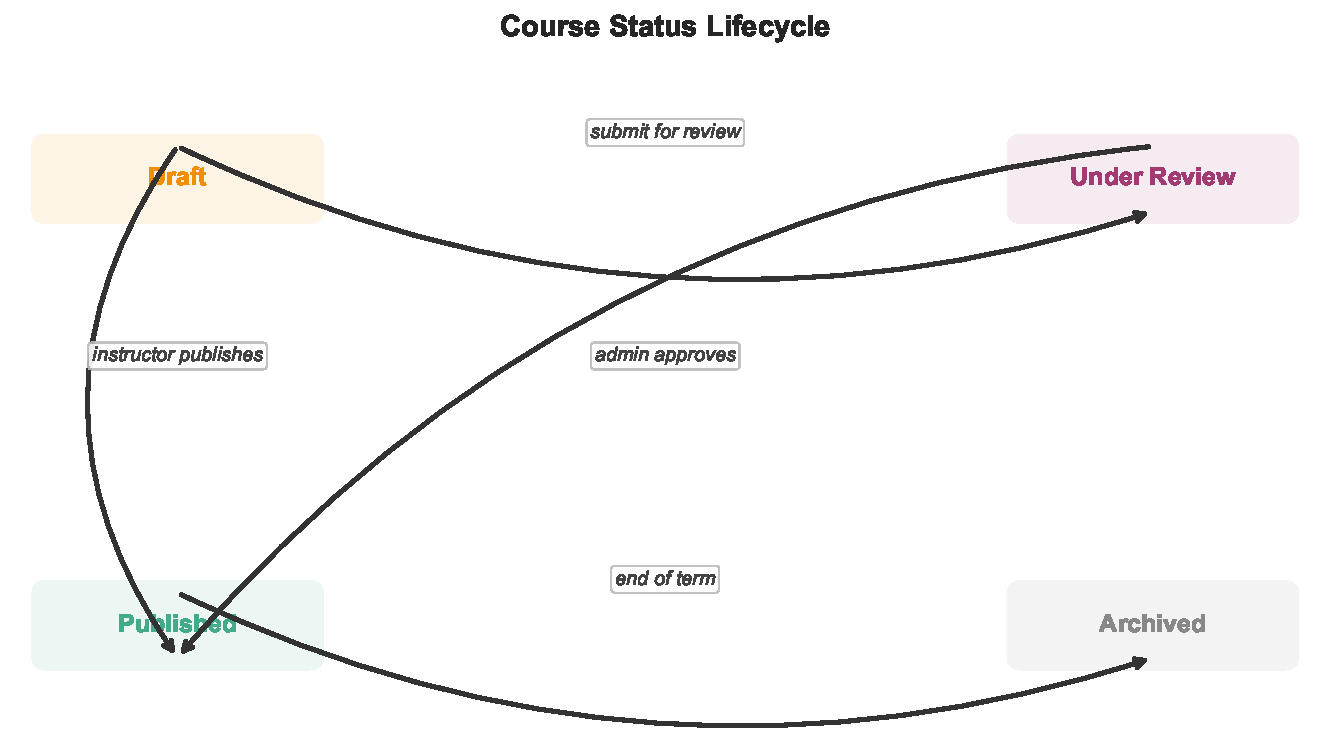
\includegraphics[width=0.55\textwidth]{images/statemachines/course_curriculum_statemachine.pdf}
  \caption{Course Status Lifecycle}
  \label{fig:course-statemachine}
\end{figure}

% =============================================================================
% Section 4.5: Media and Video Processing Module
% =============================================================================

\section{Media and Video Processing Module}
\label{sec:media-module}

\subsection{Functional Description}

The Media module manages the full lifecycle of video assets from upload to delivery. It integrates with Mux (Section~\ref{sec:video-streaming}) for transcoding, storage, and CDN delivery, while maintaining its own domain model for asset state and metadata. The module provides REST endpoints for creating direct upload URLs, querying asset status, and generating signed playback tokens for enrolled learners.

The module interacts closely with the AI Pipeline module (Section~\ref{sec:ai-pipeline-module}): when a video reaches the READY state, the Media module publishes a \texttt{VideoReady} event that triggers automatic transcript generation.

\subsection{Mux Integration and VideoAsset State Machine}

The \texttt{VideoAsset} aggregate root tracks the lifecycle of each uploaded video through the states illustrated in Figure~\ref{fig:video-statemachine}.

\begin{figure}[H]
  \centering
  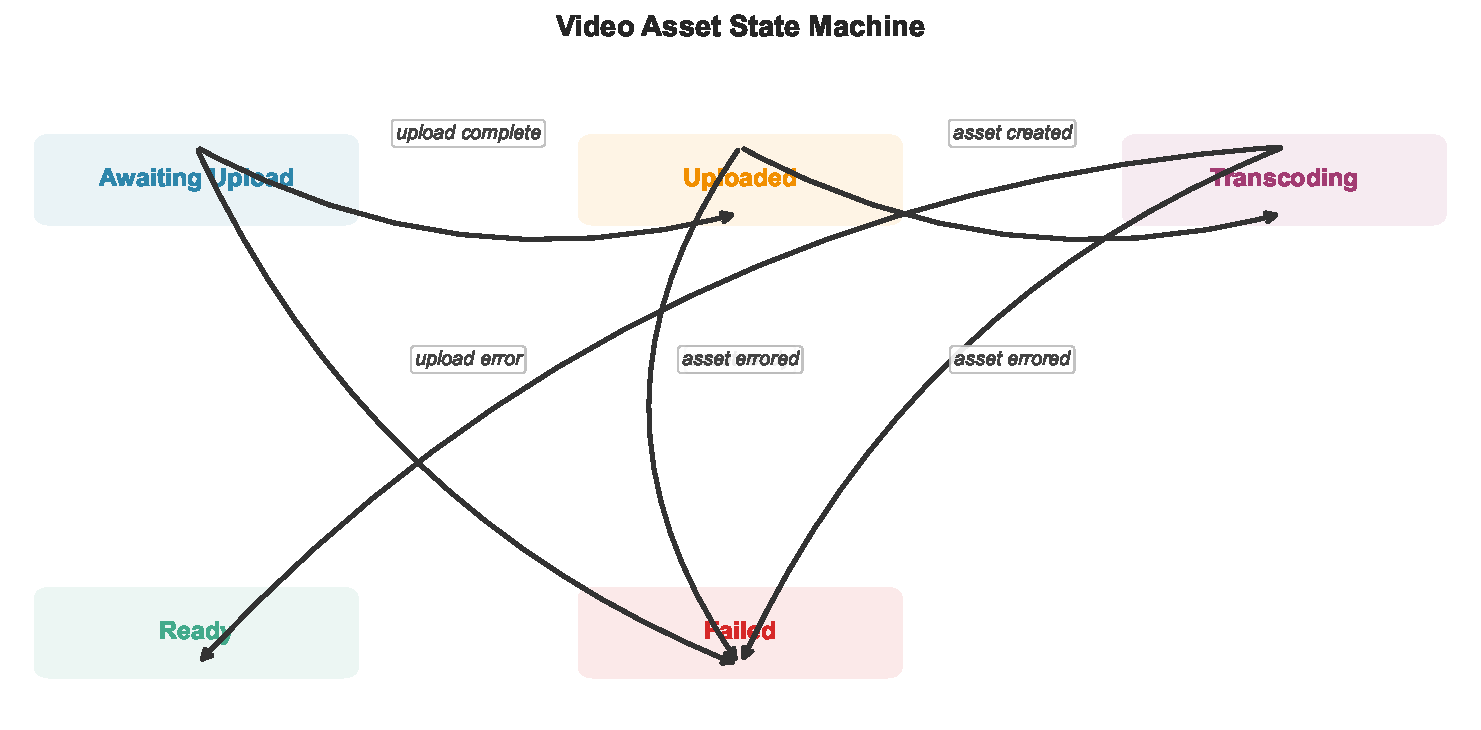
\includegraphics[width=0.75\textwidth]{images/statemachines/video_asset_statemachine.pdf}
  \caption{Video Asset State Machine}
  \label{fig:video-statemachine}
\end{figure}

The lifecycle proceeds as follows:

\begin{enumerate}
  \item \textbf{AWAITING\_UPLOAD.} A lesson is created, and an instructor calls \texttt{POST /instructor/video-assets/upload-url} to request a direct upload URL. The server calls Mux's \texttt{Upload.create()} API, obtains a signed upload URL, and stores the \texttt{upload\_id} in the \texttt{VideoAsset} entity.
  \item \textbf{UPLOADED.} The client PUTs the video file directly to Mux using the signed URL. The server does not proxy the file, avoiding bandwidth costs and latency. The state transitions to UPLOADED once Mux confirms receipt.
  \item \textbf{TRANSCODING.} Mux sends \texttt{video.upload.asset\_created}, indicating that the source file is being transcoded into HLS renditions. The Media module updates the state and creates a \texttt{GenerationJob} in the AI Pipeline module with status QUEUED.
  \item \textbf{READY.} Mux sends \texttt{video.asset.ready} with the playback ID. The Media module stores the playback ID, sets the signed URL expiry policy, and transitions the asset to READY. An outbox event \texttt{VideoReady} is published, triggering the AI pipeline to begin transcript generation.
  \item \textbf{FAILED.} Mux sends \texttt{video.asset.errored} with an error code. The state transitions to FAILED, and the instructor is notified via the Notifications module.
\end{enumerate}

\subsection{Signed Playback URL Generation}

Playback URLs are generated by the backend on request and are not stored directly. When a learner accesses a lesson, the backend verifies that the learner has an active enrollment for the course containing that lesson, then generates a JWT-signed playback URL with a 4-hour expiration:

\begin{lstlisting}[caption=Generating a Signed Mux Playback URL,label=lst:signed-url]
async function getPlaybackUrl(
  learnerId: string, lessonId: string
): Promise<string> {
  const enrollment = await this.enrollmentRepo
    .findActiveByLearnerAndLesson(learnerId, lessonId);
  if (!enrollment)
    throw new ForbiddenException('No active enrollment');

  const lesson = await this.lessonRepo.findByIdOrThrow(lessonId);
  const token = this.muxJwtService.sign({
    sub: learnerId,
    aud: `playback:${lesson.videoAsset.playbackId}`,
    exp: Math.floor(Date.now() / 1000) + 14400, // 4 hours
  });

  return `https://stream.mux.com/${lesson.videoAsset.playbackId}.m3u8?token=${token}`;
}
\end{lstlisting}

This design ensures that: (1) learners cannot share playback URLs beyond the 4-hour window; (2) revoked enrollments are immediately reflected---the next request generates a playback URL only if the enrollment is still active; and (3) unauthorised users never receive a valid playback URL because the authorization check happens server-side before the JWT is signed.

Figure~\ref{fig:seq-video-streaming} illustrates the end-to-end flow. The instructor uploads a video through the Media module, which obtains a Mux upload URL without proxying the file. The client uploads directly to Mux. Asynchronous webhooks drive the state machine: \texttt{video.upload.asset\_created} transitions to UPLOADED and then TRANSCODING; \texttt{video.asset.ready} transitions to READY and stores the playback ID. When a learner later requests the lesson content, the server verifies the learner has an active enrollment, generates a signed JWT playback URL with a 4-hour expiry, and the client streams HLS segments directly from the Mux CDN.

\begin{figure}[H]
  \centering
  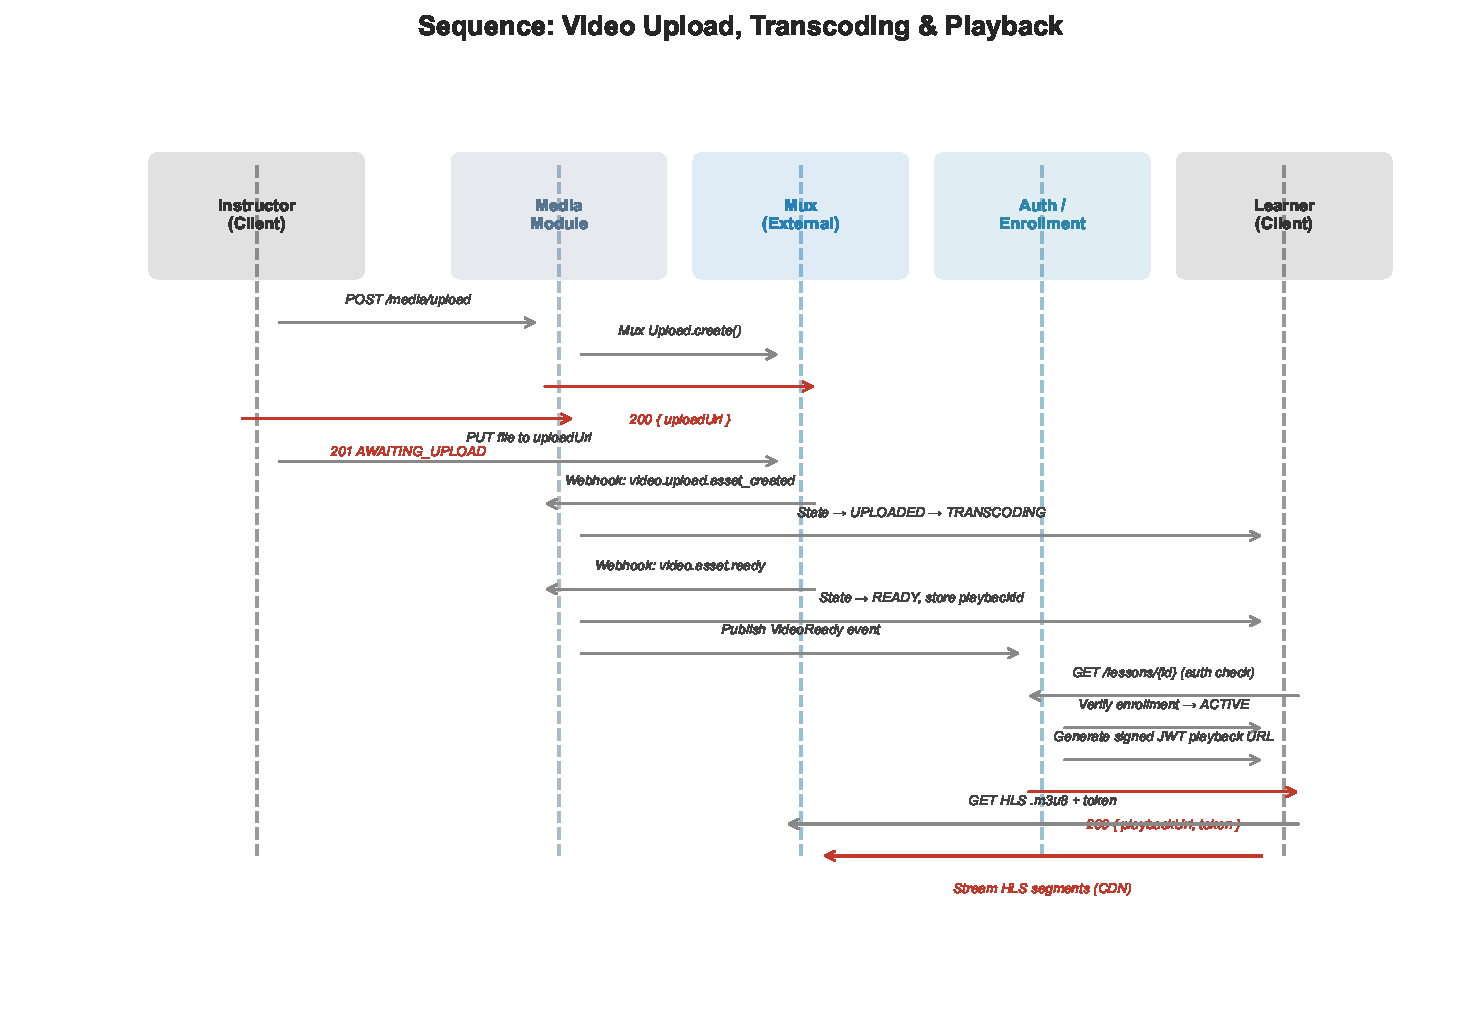
\includegraphics[width=0.85\textwidth]{images/seq_video_streaming.pdf}
  \caption{Sequence Diagram: Video Upload, Transcoding \& Playback}
  \label{fig:seq-video-streaming}
\end{figure}

% =============================================================================
% Section 4.6: AI Pipeline Integration Module
% =============================================================================

\section{AI Pipeline Integration Module}
\label{sec:ai-pipeline-module}

\subsection{Functional Description}

The AI Pipeline module orchestrates the automated generation of transcripts and quiz questions from video content using external AI services. It exposes internal-use-only endpoints for AI service callbacks (HMAC-authenticated) and publishes domain events that trigger notifications for instructor review. The module manages two distinct workflows: \textbf{transcript generation} (Whisper ASR) and \textbf{quiz generation} (LLM).

Both workflows follow an asynchronous callback pattern: NexaLearn dispatches a request to the AI service (via HTTP or queue), the service processes the job, and the service calls back a NexaLearn endpoint with the result. This decouples processing time---transcribing a 60-minute lecture may take several minutes---from the API response time.

\subsection{HMAC Signature Verification}

All callbacks from the AI pipeline include an \texttt{X-Pipeline-Signature} header with format \texttt{t=<unix-timestamp>,v1=<hex-digest>}. The recipient controller verifies the signature before processing:

\begin{lstlisting}[caption=HMAC Callback Verification,label=lst:hmac-verify]
@Post('callbacks/transcript')
async handleTranscriptCallback(
  @Headers('x-pipeline-signature') signature: string,
  @Body() payload: TranscriptCallbackDto,
): Promise<void> {
  this.hmacService.verify(signature, payload);
  await this.useCase.execute(payload);
}

// In HmacService
verify(signature: string, body: unknown): void {
  const [tsPart, hashPart] = signature.split(',');
  const timestamp = parseInt(tsPart.replace('t=', ''), 10);
  const receivedHash = hashPart.replace('v1=', '');

  if (Math.abs(Date.now() / 1000 - timestamp) > 300)
    throw new SecurityException('Callback timestamp expired');

  const computed = createHmac('sha256', this.secret)
    .update(`${timestamp}.${JSON.stringify(body)}`)
    .digest('hex');

  if (!timingSafeEqual(computed, receivedHash))
    throw new SecurityException('HMAC signature mismatch');
}
\end{lstlisting}

The timestamp tolerance (300 seconds) prevents replay attacks without requiring clock synchronisation tighter than typical NTP guarantees. The \texttt{timingSafeEqual} comparison prevents timing side-channel attacks.

\subsection{HandleGenerationCallbackUseCase --- Exactly-Once Processing}

The callback handler must be idempotent: the AI service may retry callbacks if it does not receive a 200 response. The \texttt{HandleGenerationCallbackUseCase} uses the \texttt{GenerationJob} aggregate to ensure each callback is processed exactly once:

\begin{lstlisting}[caption=Exactly-Once Callback Processing,label=lst:exactly-once]
async execute(dto: TranscriptCallbackDto): Promise<void> {
  await this.prisma.$transaction(async (tx) => {
    const job = await tx.generationJob.findUniqueOrThrow({
      where: { id: dto.jobId },
    });

    if (job.status !== 'PROCESSING') return; // already processed

    await tx.generationJob.update({
      where: { id: dto.jobId },
      data: {
        status: 'CALLBACK_RECEIVED',
        result: dto.transcript,
        completedAt: new Date(),
      },
    });

    await tx.outboxEvent.create({
      data: {
        aggregateType: 'GenerationJob',
        aggregateId: dto.jobId,
        eventType: 'TranscriptGenerated',
        payload: { transcript: dto.transcript, videoAssetId: job.videoAssetId },
      },
    });
  });
}
\end{lstlisting}

The guard clause (\texttt{if (job.status !== 'PROCESSING') return}) ensures that if the same callback arrives twice, the second invocation is a no-op. The outbox event triggers downstream handlers that create the \texttt{GeneratedQuiz} record (if quiz generation is enabled) and notify the instructor.

\subsection{Quiz Review Workflow}

Generated quizzes transition through three statuses: \texttt{READY\_FOR\_REVIEW} (initial, awaiting instructor action), \texttt{APPROVED} (instructor accepted), and \texttt{REJECTED} (instructor rejected with feedback). The instructor reviews each proposed question in a dashboard, edits the stem or options, and either approves or rejects the entire quiz. Only upon approval does the quiz become available to learners. This human-in-the-loop workflow, illustrated in Figure~\ref{fig:ai-job-statemachine}, ensures quality control without requiring the instructor to author questions from scratch.

\begin{figure}[H]
  \centering
  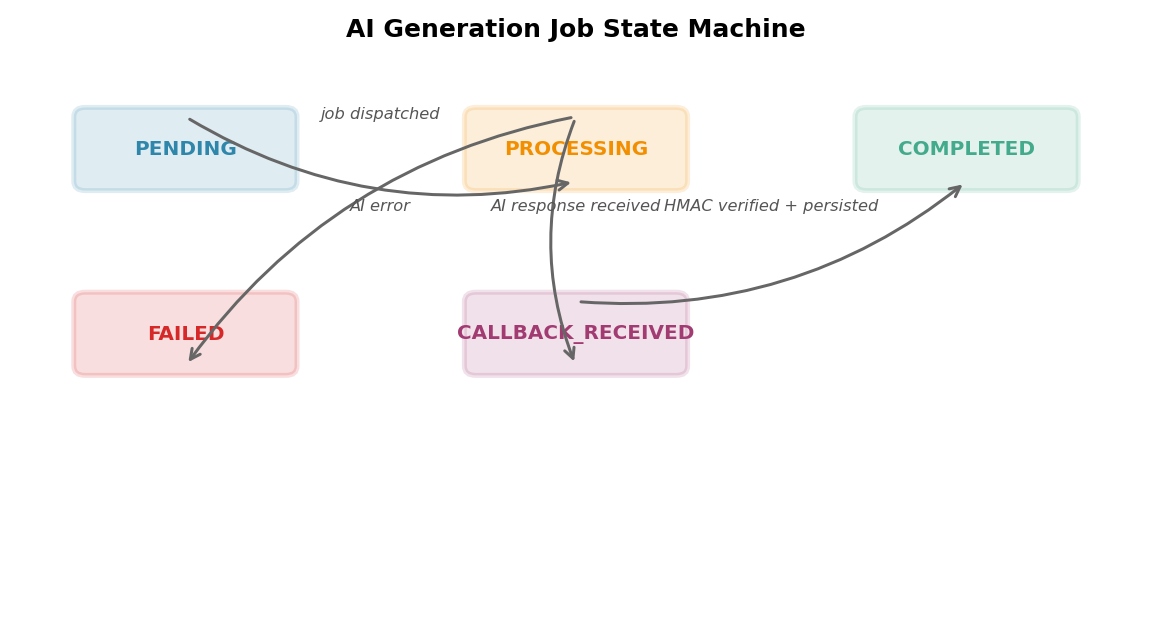
\includegraphics[width=0.7\textwidth]{images/statemachines/ai_job_statemachine.png}
  \caption{AI Generation Job State Machine}
  \label{fig:ai-job-statemachine}
\end{figure}

% =============================================================================
% Section 4.7: Assessment and Quiz Module
% =============================================================================

\section{Assessment and Quiz Module}
\label{sec:assessment-module}

\subsection{Functional Description}

The Assessment module is one of the most domain-rich contexts in NexaLearn. It manages the full lifecycle of quizzes, questions, and learner attempts. The module supports multiple question types (multiple-choice, true-or-false, short-answer), configurable passing scores, time limits, randomisation, and both automatic and AI-assisted (short-answer) grading. Quiz results feed into the Progress module for learner analytics and into the Reviews module for peer assessment of short-answer responses.

\subsection{Quiz Authoring Aggregate}

The \texttt{QuizEntity} aggregate root enforces the invariants of quiz authoring:

\begin{lstlisting}[caption=QuizEntity Aggregate Root Showing Invariants,label=lst:quiz-entity]
export class QuizEntity {
  constructor(
    public readonly id: string,
    public lessonId: string,
    public title: string,
    public instructions: string,
    public passingScore: number,       // 0--100
    public maxAttempts: number,         // 0 = unlimited
    public timeLimitMinutes: number | null,
    public shuffleQuestions: boolean,
    public questions: QuestionEntity[],
    public status: QuizStatus,
  ) {}

  addQuestion(question: QuestionEntity): void {
    if (this.status !== QuizStatus.DRAFT)
      throw new BusinessRuleViolation('Cannot modify published quiz');
    this.questions.push(question);
  }

  publish(): void {
    if (this.questions.length < 1)
      throw new BusinessRuleViolation('Quiz must have at least 1 question');
    if (this.questions.some(q => q.options.length < 2))
      throw new BusinessRuleViolation('Each question needs at least 2 options');
    this.status = QuizStatus.PUBLISHED;
  }

  gradeAttempt(
    answers: AnswerDto[],
    shortAnswerGradingService: ShortAnswerGradingService,
  ): QuizAttemptEntity {
    let correctCount = 0;
    const gradedAnswers = answers.map((answer) => {
      const question = this.questions.find(q => q.id === answer.questionId);
      if (!question) throw new BusinessRuleViolation('Question not found');

      if (question.type === QuestionType.SHORT_ANSWER) {
        return {
          questionId: question.id,
          status: 'PENDING_GRADING',
          pointsAwarded: null,
        };
      }

      const isCorrect = question.correctOptionId === answer.selectedOptionId;
      if (isCorrect) correctCount++;
      return {
        questionId: question.id,
        selectedOptionId: answer.selectedOptionId,
        isCorrect,
        pointsAwarded: isCorrect ? question.points : 0,
      };
    });

    const score = Math.round((correctCount / this.questions.length) * 100);
    const passed = score >= this.passingScore;

    const hasPendingGrading = gradedAnswers.some(a => a.status === 'PENDING_GRADING');

    return QuizAttemptEntity.create({
      quizId: this.id,
      answers: gradedAnswers,
      score,
      passed,
      status: hasPendingGrading ? QuizAttemptStatus.IN_PROGRESS : QuizAttemptStatus.GRADED,
    });
  }
}
\end{lstlisting}

The aggregate root is the sole authority for grading: it receives learner answers, computes scores by comparing against the correct option for each multiple-choice question, and flags short-answer questions for asynchronous AI grading.

\subsection{Quiz Attempt Lifecycle}

Figure~\ref{fig:quiz-attempt-statemachine} shows the states of a quiz attempt.

\begin{figure}[H]
  \centering
  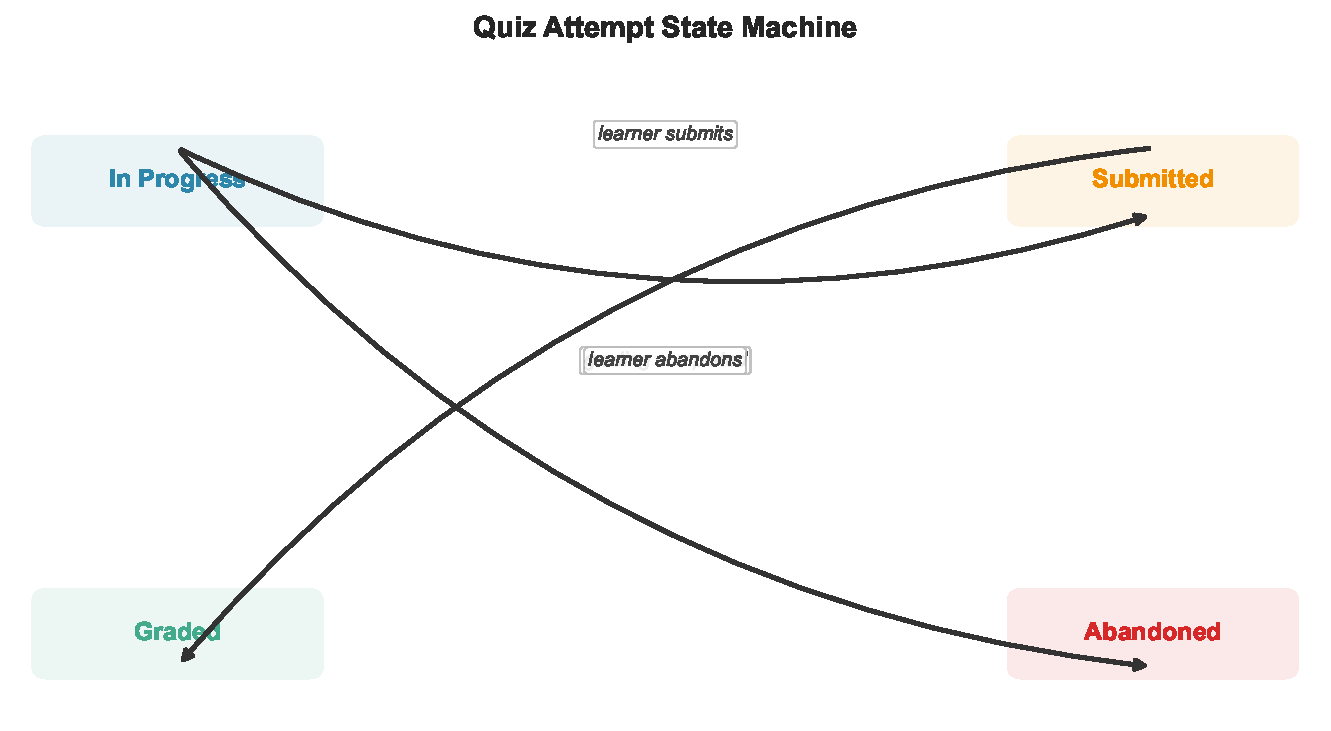
\includegraphics[width=0.7\textwidth]{images/statemachines/quiz_attempt_statemachine.pdf}
  \caption{Quiz Attempt State Machine}
  \label{fig:quiz-attempt-statemachine}
\end{figure}

When a learner starts a quiz, an attempt is created in IN\_PROGRESS state with a snapshot of the quiz questions (ensuring the quiz cannot change mid-attempt). When the learner submits, the attempt transitions to SUBMITTED. If all questions are auto-gradable (multiple-choice, true-or-false), the attempt is graded synchronously and transitions to GRADED. If the quiz includes short-answer questions, the attempt remains in SUBMITTED while the grading callback is awaited. When the AI pipeline responds, the attempt transitions to GRADED and the updated score is persisted. Learners may also abandon an attempt, transitioning it to ABANDONED.

\subsection{Asynchronous Short-Answer Grading}

Short-answer questions cannot be graded by simple string comparison---the learner's answer may be semantically correct regardless of exact wording. The Assessment module delegates grading to an LLM (configured per deployment as OpenAI GPT-4 or a self-hosted alternative). The grading prompt includes the question stem, the instructor-provided rubric, and the learner's answer, and returns a grade (0--100), a justification, and optionally feedback for the learner. The grader endpoint is call-back authenticated using the same HMAC pattern described in Section~\ref{sec:ai-pipeline-module}. Until grading completes, the learner sees a ``Grading in progress'' status. When grading finishes, the learner is notified, and the updated score propagates to the Progress module via an outbox event.

% =============================================================================
% Section 4.8: Payment Module
% =============================================================================

\section{Payment Module}
\label{sec:payment-module}

\subsection{Functional Description}

The Payment module manages the lifecycle of financial transactions between learners and the platform. It integrates with Stripe for payment processing and webhook delivery, maintains its own payment intent state machine for reconciliation, and coordinates with the Enrollment module to activate course access only after successful payment. The module also handles refunds, partial payments, and coupon applications.

The module is designed to be Stripe-agnostic at the domain layer: the PaymentIntent aggregate and its state machine use a generic set of states and commands. A dedicated StripeInfrastructureService maps Stripe-specific constructs (PaymentIntent API objects, webhook event types) to the domain model, allowing the payment provider to be swapped without modifying domain logic.

\subsection{Stripe Integration and Webhook Handling}

Checkout flow proceeds as follows:

\begin{enumerate}
  \item The client requests \texttt{POST /api/payments/create-checkout} with course ID and learner ID. The Payment module creates a Stripe Checkout Session via the Stripe SDK and returns the session URL to the client.
  \item The client redirects the learner to Stripe's hosted checkout page. The learner completes payment on Stripe's domain, which reduces PCI-DSS compliance scope for the platform.
  \item Stripe sends a \texttt{checkout.session.completed} webhook to NexaLearn's \texttt{POST /api/payments/stripe-webhook}. The webhook handler verifies the Stripe signature using \texttt{stripe.webhooks.constructEvent()}, retrieves the session details, and invokes the \texttt{HandlePaymentSucceededUseCase}.
  \item The use case loads or creates a \texttt{PaymentIntent} aggregate, transitions it to SUCCEEDED, and publishes a \texttt{PaymentSucceeded} outbox event. The Enrollment module's event handler creates or activates the corresponding enrollment.
\end{enumerate}

Webhook idempotency is critical---Stripe may deliver the same webhook event multiple times. Stripe events include a unique \texttt{idempotency\_key} in their HTTP header; NexaLearn records processed webhook IDs in a ledger table and ignores duplicates:

\begin{lstlisting}[caption=Idempotent Stripe Webhook Processing,label=lst:stripe-idempotent]
async function handleWebhook(event: Stripe.Event): Promise<void> {
  const processed = await this.webhookLedger.findUnique({
    where: { stripeEventId: event.id },
  });
  if (processed) return; // already handled

  await this.prisma.$transaction(async (tx) => {
    await tx.webhookLedger.create({
      data: { stripeEventId: event.id, processedAt: new Date() },
    });
    // process event...
  });
}
\end{lstlisting}

\subsection{Payment Intent State Machine}

Figure~\ref{fig:payment-statemachine} shows the PaymentIntent state machine.

\begin{figure}[H]
  \centering
  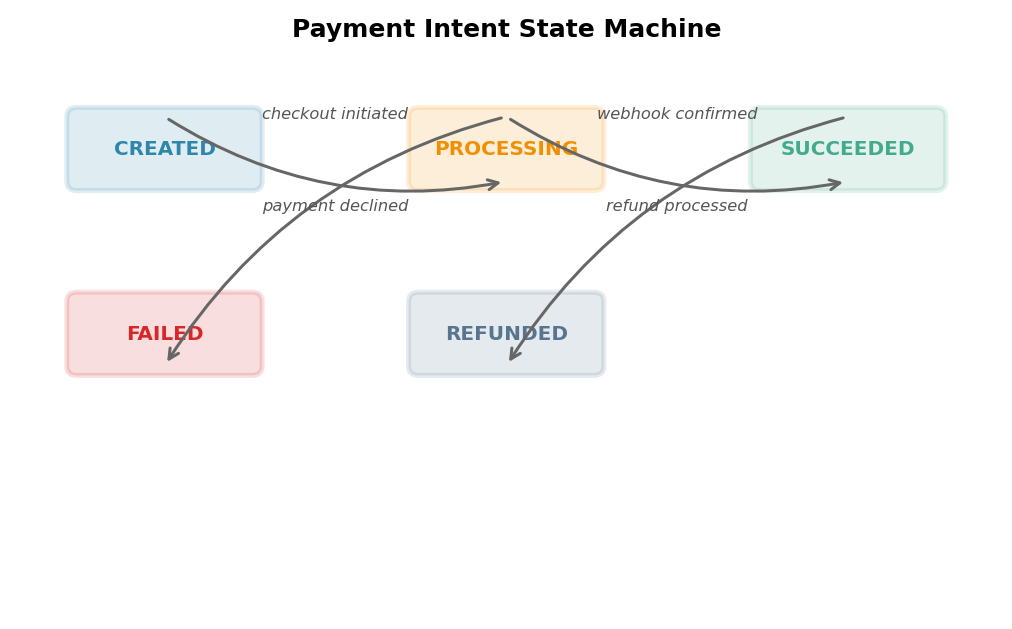
\includegraphics[width=0.65\textwidth]{images/statemachines/payment_intent_statemachine.png}
  \caption{Payment Intent State Machine}
  \label{fig:payment-statemachine}
\end{figure}

The \texttt{PaymentIntent} aggregate transitions through states: CREATED when the checkout session is initiated, PROCESSING while awaiting Stripe confirmation, SUCCEEDED upon confirmed payment, FAILED if the payment was declined or expired, and REFUNDED when a succeeded payment is refunded. Each transition is recorded as an immutable \texttt{PaymentEvent} in a separate event table, providing an audit trail for financial reconciliation.

\subsection{Reconciliation and Expiration Services}

Two scheduled services handle edge cases in the payment lifecycle:

\begin{description}
  \item[\textbf{ReconciliationService.}] Runs daily and retrieves all PaymentIntents in PROCESSING state older than 24 hours. It queries Stripe for the latest status of each associated Checkout Session and updates the local state accordingly, handling cases where the webhook was never delivered (e.g., network outage).
  \item[\textbf{ExpirationService.}] Runs hourly and expires Checkout Sessions older than 24 hours. This garbage-collects abandoned payment flows and releases any temporary holds on inventory or enrollment slots.
\end{description}

Both services are implemented as NestJS \texttt{@Cron} decorators with configurable cron expressions and are disabled in test environments.

% =============================================================================
% Section 4.9: Enrollment Module
% =============================================================================

\section{Enrollment Module}
\label{sec:enrollment-module}

\subsection{Free vs. Paid Enrollment Flow}

The Enrollment module manages how learners gain access to courses. Two enrollment flows exist:

\begin{description}
  \item[\textbf{Free enrollment.}]
  If a course price is zero, the enrollment is created and activated immediately within a single database transaction. The EnrollmentController invokes \texttt{CreateFreeEnrollmentUseCase}, which creates the \texttt{Enrollment} aggregate in ACTIVE state and publishes an \texttt{EnrollmentActivated} event. This event triggers the Progress module to initialise the learner's progress projections for all lessons in the course curriculum.

  \item[\textbf{Paid enrollment.}]
  If a course has a non-zero price, the enrollment is created in PENDING state. The Enrollment module does not handle payment directly; it waits for an outbound event from the Payment module. When \texttt{PaymentSucceeded} is consumed by the \texttt{OnPaymentSucceeded} event handler in the Enrollment module, the handler loads the corresponding enrollment (matched by a correlation ID stored in the Stripe Checkout Session metadata), activates it, and publishes \texttt{EnrollmentActivated}.
\end{description}

The explicit separation of free and paid paths ensures that paid enrollments cannot accidentally be activated without payment confirmation through the Payment module's state machine.

\subsection{Idempotency and Concurrent Enrollment Protection}

Enrollment creation is protected against concurrent requests. The \texttt{CreateEnrollmentUseCase} checks for an existing active enrollment before creating a new one:

\begin{lstlisting}[caption=Concurrent Enrollment Protection,label=lst:enrollment-idempotent]
async execute(dto: CreateEnrollmentDto): Promise<Enrollment> {
  return this.prisma.$transaction(async (tx) => {
    const existing = await tx.enrollment.findFirst({
      where: {
        learnerId: dto.learnerId,
        courseId: dto.courseId,
        status: { in: ['ACTIVE', 'COMPLETED'] },
      },
    });

    if (existing) {
      if (dto.idempotencyKey) return existing;
      throw new BusinessRuleViolation('Already enrolled in this course');
    }

    const enrollment = EnrollmentEntity.create(
      dto.learnerId, dto.courseId,
      dto.price > 0 ? EnrollmentStatus.PENDING : EnrollmentStatus.ACTIVE,
    );

    await tx.enrollment.create({ data: this.mapToPersistence(enrollment) });

    if (enrollment.isActive) {
      await tx.outboxEvent.create({
        data: {
          aggregateType: 'Enrollment',
          aggregateId: enrollment.id,
          eventType: 'EnrollmentActivated',
          payload: { learnerId: dto.learnerId, courseId: dto.courseId },
        },
      });
    }

    return enrollment;
  });
}
\end{lstlisting}

The \texttt{findFirst} lookup with status filter uses a composite index on \texttt{(learnerId, courseId, status)} for efficient querying. The entire operation---check, create, insert outbox event---occurs within a single Prisma transaction, preventing race conditions where two concurrent requests could both pass the existence check.

Figure~\ref{fig:enrollment-statemachine} shows the enrollment lifecycle.

\begin{figure}[H]
  \centering
  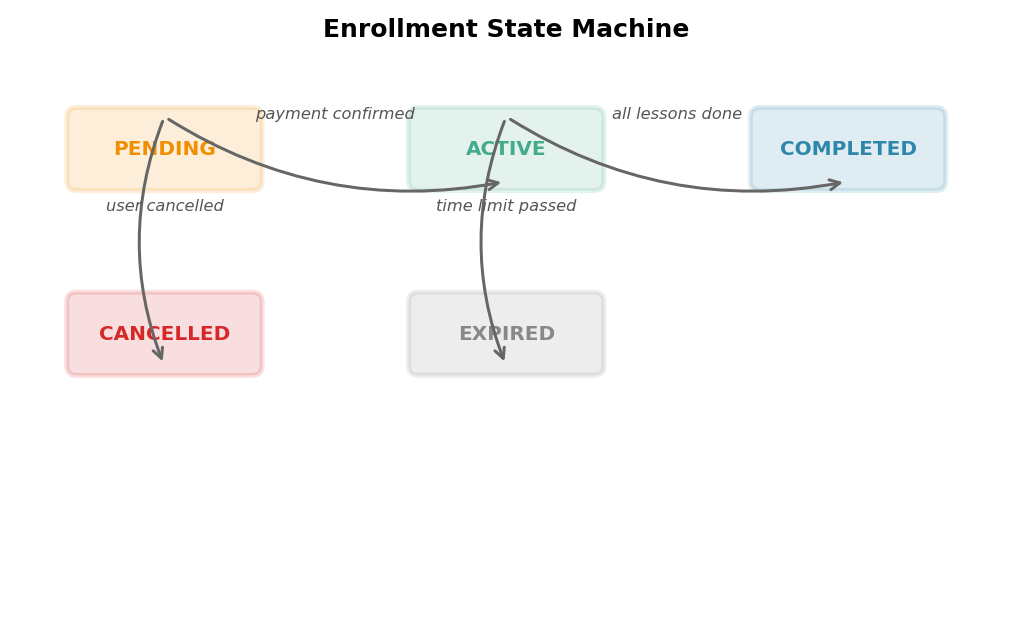
\includegraphics[width=0.6\textwidth]{images/statemachines/enrollment_statemachine.png}
  \caption{Enrollment State Machine}
  \label{fig:enrollment-statemachine}
\end{figure}

Enrollments transition from PENDING to ACTIVE (payment confirmed or free enrollment), from ACTIVE to COMPLETED (all curriculum requirements satisfied), from PENDING to CANCELLED (learner abandoned checkout or manually cancelled), and from ACTIVE to EXPIRED (course access duration limit exceeded, if configured).

% =============================================================================
% Section 4.10: Discussion and Q&A Module
% =============================================================================

\section{Discussion and Q\&A Module}
\label{sec:discussion-module}

\subsection{Thread and Post Aggregate Design}

The Discussion module implements a tree-structured thread-and-post model common to forum and Q\&A systems. The aggregate root is \texttt{ThreadEntity}, which is scoped to a specific lesson (per-lesson discussion) or to a course (general discussion). A thread has a title, a creator (learner or instructor), a collection of \texttt{PostEntity} children, and a lifecycle status.

The aggregate enforces the forum structure invariants:

\begin{lstlisting}[caption=Discussion Thread Aggregate,label=lst:thread-aggregate]
export class ThreadEntity {
  constructor(
    public readonly id: string,
    public readonly courseId: string,
    public readonly lessonId: string | null,
    public readonly creatorId: string,
    public title: string,
    public body: string,
    public isPinned: boolean,
    public isResolved: boolean,
    public isHidden: boolean,
    public posts: PostEntity[],
    public createdAt: Date,
    public updatedAt: Date,
  ) {}

  addPost(learnerId: string, body: string): PostEntity {
    if (this.isHidden)
      throw new BusinessRuleViolation('Thread is closed');
    if (body.length > 5000)
      throw new BusinessRuleViolation('Post exceeds 5000 characters');

    const post = PostEntity.create({
      threadId: this.id,
      authorId: learnerId,
      body,
    });

    this.posts.push(post);
    this.updatedAt = new Date();
    return post;
  }

  markResolved(): void {
    this.isResolved = true;
    this.updatedAt = new Date();
  }
}
\end{lstlisting}

When a post is added by an instructor to a learner's thread, the \texttt{InstructorReplied} domain event is published. This event is consumed by the Notifications module, which sends an email notification to the thread creator. The notification includes a direct link to the thread in the learner dashboard.

\subsection{Instructor Reply Notifications}

Notification flow: \texttt{ThreadEntity.addPost()} creates a \texttt{PostEntity} and marks the thread as updated. The \texttt{AddPostUseCase} persists the thread and post, then publishes an outbox event. The Notifications module's event handler checks whether the author of the new post has the \texttt{instructor} role on the course. If so, it creates a \texttt{Notification} entity for each learner who has posted in the thread, containing the instructor's reply excerpt and a link to the thread. Notifications are delivered via Resend transactional email and are also accessible via the NexaLearn REST API for in-app notification display.

Figure~\ref{fig:discussion-statemachine} illustrates the thread lifecycle using boolean flags: a thread is open by default, marked as resolved by the instructor, or hidden through moderation.

\begin{figure}[H]
  \centering
  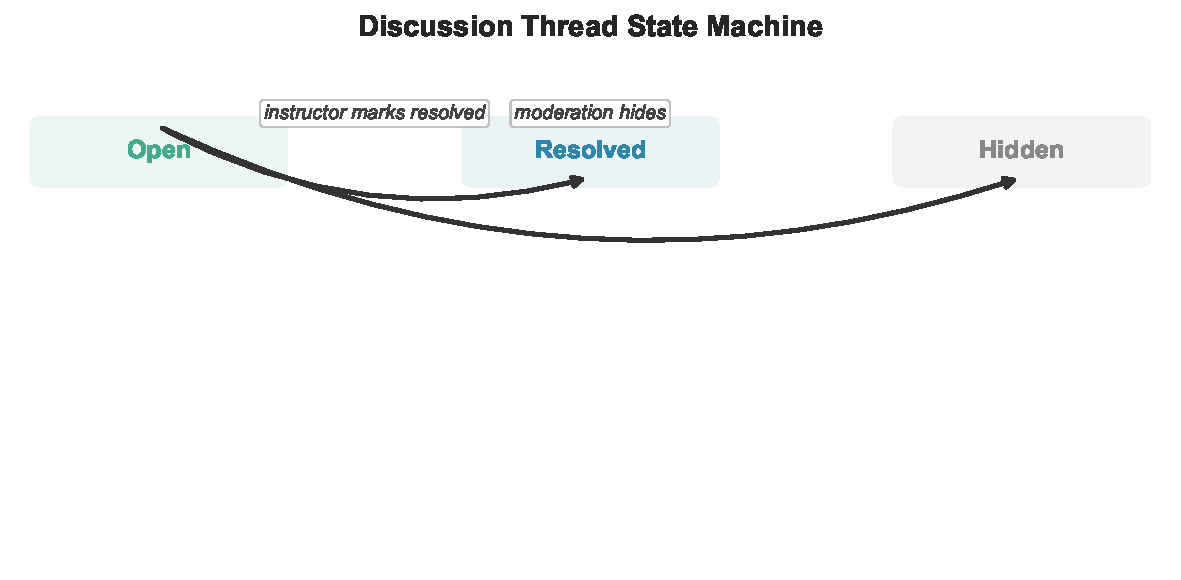
\includegraphics[width=0.5\textwidth]{images/statemachines/discussion_statemachine.pdf}
  \caption{Discussion Thread State Machine}
  \label{fig:discussion-statemachine}
\end{figure}

% =============================================================================
% Section 4.11: Security Design
% =============================================================================

\section{Security Design}
\label{sec:security-design}

\subsection{HMAC Service-to-Service Authentication}

NexaLearn uses HMAC-based authentication for internal service-to-service communication when external webhook callbacks are received. Three external services authenticate via HMAC: Stripe (webhook signatures using \texttt{stripe-webhook-secret}), Mux (webhook signatures using \texttt{mux-webhook-secret}), and the AI Pipeline (custom HMAC using a shared secret configured per deployment).

The implementation uses a generic \texttt{HmacGuard} NestJS guard that extracts the signature from the request header, computes the expected HMAC using the request body and the configured secret for the service, and rejects requests that do not match within a time-tolerance window:

\begin{lstlisting}[caption=Generic HMAC Webhook Guard,label=lst:hmac-guard]
@Injectable()
export class HmacWebhookGuard implements CanActivate {
  constructor(
    private readonly configService: ConfigService,
    private readonly provider: 'stripe' | 'mux' | 'ai-pipeline',
  ) {}

  async canActivate(context: ExecutionContext): Promise<boolean> {
    const request = context.switchToHttp().getRequest();
    const signature = request.headers[this.headerName()] as string;
    const body = JSON.stringify(request.body);

    if (!signature) return false;

    const secret = this.configService.get<string>(
      `${this.provider}_WEBHOOK_SECRET`
    );

    return this.verify(signature, body, secret);
  }

  private verify(signature: string, body: string, secret: string): boolean {
    // Provider-specific verification (Stripe SDK, Mux SDK, or custom HMAC)
    // ...
  }
}
\end{lstlisting}

This guards can be applied to specific controller routes via NestJS decorators: \texttt{@UseGuards(new HmacWebhookGuard('stripe'))}.

\subsection{Rate Limiting}

NexaLearn implements distributed rate limiting using the \texttt{@nestjs/throttler} module with a Redis-backed storage adapter. The rate limiter tracks request counts per IP address and per authenticated user ID, with separate limits for read endpoints (100 requests per minute per user) and write endpoints (20 requests per minute per user). Exceeding the limit returns HTTP 429 Too Many Requests with a \texttt{Retry-After} header.

The Redis-backed ThrottlerModule uses a sliding window algorithm: each request increments a counter in Redis with a TTL equal to the window duration, and counters are checked before allowing the request. This design ensures that rate limits are consistent across multiple application instances (which is essential for the modular monolith if horizontally scaled behind a load balancer).

Additional throttling is applied to sensitive endpoints: login (5 attempts per minute per IP), password reset (3 attempts per hour per user), and AI pipeline callbacks (no rate limit for internal callbacks, but validated by HMAC).

\subsection{Audit Logging}

The Audit module provides an immutable, queryable log of all state-changing operations across the platform. Each audit entry records:

\begin{itemize}
  \item \textbf{Actor.} The user ID and role that performed the operation (or \texttt{SYSTEM} for automated actions).
  \item \textbf{Action.} A canonical action name (e.g., \texttt{enrollment.activate}, \texttt{course.publish}, \texttt{payment.refund}).
  \item \textbf{Resource.} The aggregate type and ID affected by the action.
  \item \textbf{Context.} The request IP, user agent, and correlation ID (propagated via a NestJS middleware that assigns a UUID to each incoming HTTP request).
  \item \textbf{Diff.} A JSON snapshot of the relevant aggregate state before and after the operation (optional, configurable per action type).
\end{itemize}

Audit entries are written to a dedicated \texttt{audit\_log} PostgreSQL table. Writes are fire-and-forget (no outbox): if the audit write fails, the primary operation is not rolled back. This trade-off---audit loss in rare failure scenarios versus operational complexity---is acceptable because the financial trail is already guaranteed by the Payment module's event ledger.

The audit log is exposed to administrators via a read-only REST endpoint with pagination and filtering by actor, action, resource type, and date range. Retention is configurable; the default policy retains audit logs for one year, after which they are archived to cold storage.

